\begin{figure*}[t!]
    \centering
    \begin{subfigure}[t]{0.78\linewidth}
        \centering
        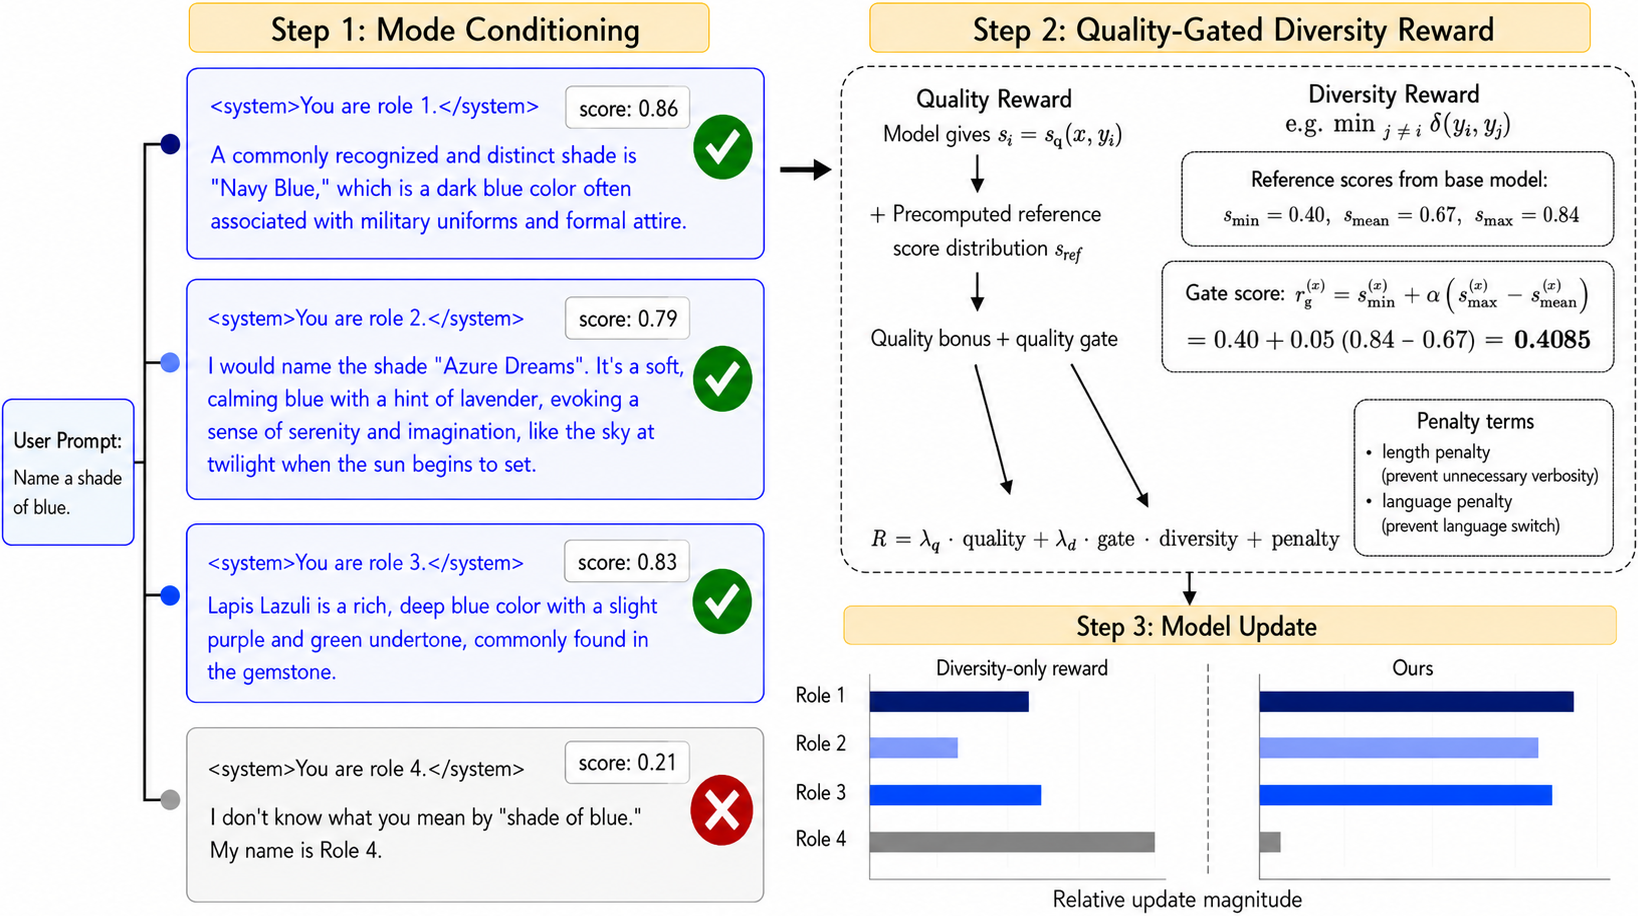
\includegraphics[width=\textwidth]{figures/method_v3.png}
        \label{fig:architecture}
    \end{subfigure}\hfill
    \begin{subfigure}[t]{0.2\linewidth}
        \centering
        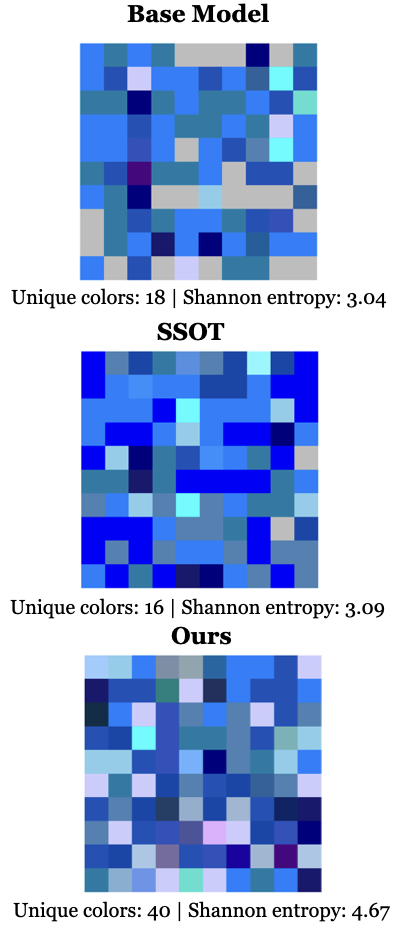
\includegraphics[width=\linewidth]{figures/blue.png}
        \label{fig:40blue}
    \end{subfigure}
    \vspace{-0.2cm}
\caption{\textbf{Left}: Overview of \method. \method{} uses mode conditioning to elicit diverse candidate responses, then applies a quality-gated diversity reward with penalty terms to promote high-quality diversity. Each candidate is labeled with its quality score $s_i$ relative to the prompt-adaptive quality threshold $\tau_q^{(x)}$. Candidates with $s_i<\tau_q^{(x)}$ have $g(x,y_i)=0$ and therefore receive no diversity credit. Step 3 shows the resulting signed group-relative advantages $\widehat{A}_i$; positive advantages promote a response, whereas negative advantages suppress it during the policy update. Matching colors track the same response through Steps 1--3. \textbf{Right}: 100 responses to the prompt \textbf{``Name a shade of blue''} from the Qwen3-8B initial policy (\texttt{Qwen/Qwen3-8B}), String Seed of Thought (\ssot)~\citep{Misaki2026}, and \method{} under diverse-mode inference. \method{} produces 40 distinct shades of blue, 122\% more than the Qwen3-8B initial policy and 150\% more than \ssot. \liweiaddressed{It's unclear what the two bar charts of Model update mean? I think the issue is that, it's not intuitive which of the four generations in Step 1 is considered low quality, and hence needs penalty. One possibility is to add in the quality score (mock-up is fine), to the upper-right corner of each generation box, plus, provide a reference score. So that it makes it more clear which response should be suppressed during model update. Also the four bars in Step 3 seem to have different colors compared to the four boxes in Step 1. }
}
\label{fig:moda + 40blue}
\end{figure*}


\section{Introduction}
\label{sec:introduction}

Post-training alignment is essential for improving the capability and safety of large language models (LLMs), but it also introduces a concerning side effect: \textit{mode collapse}. Aligned models increasingly favor a narrow set of responses (the ``mode'') over the broader space of plausible outputs, resulting in a substantial loss of generation diversity~\citep{jiang2025artificialhivemindopenendedhomogeneity, west2025base, huang2024self, sourati2026homogenizingeffectlargelanguage}. Yet in many domains, diversity is not merely desirable but essential. In AI-assisted scientific discovery, progress relies on exploring a broad and plausible hypothesis space rather than prematurely converging on a single line of inquiry~\citep{gruver2023proteindesignguideddiscrete, romera2024mathematical}. Likewise, generative diversity is critical for applications requiring creativity and open-ended exploration~\citep{Shumailov2024AIMC, abdulhai2026llmsdistortwrittenlanguage}. While inference-time interventions~\citep{Misaki2026, Zhang2025} can partially mitigate this loss of diversity, a more fundamental solution is to redesign post-training algorithms so that expressivity is preserved throughout the alignment process by construction.

We introduce \method~(\textbf{Mo}de-conditioned \textbf{D}iversity \textbf{A}lignment), an online post-training RL algorithm that jointly optimizes the quality and diversity of generated responses by formulating alignment through the lens of multi-agent reinforcement learning (MARL), where agents develop diverse behaviors through competition and coordination~\citep{eysenbach2018diversityneedlearningskills,liang2024learning,li2021celebratingdiversitysharedmultiagent}. \method{} introduces \textit{role conditioning} to instantiate multiple lightweight agents within a single shared policy. Specifically, we prepend abstract role tokens to the system prompt, enabling each role to generate a response to the same user query while independently optimizing a group-relative diversity reward. This creates competitive reward dynamics among roles, encouraging them to specialize in distinct regions of the high-quality response space and collectively produce a diverse set of outputs.

A key design choice of \method{} is a \textit{prompt-adaptive quality gate} that grants diversity rewards only to responses exceeding a prompt-specific quality threshold computed from a frozen reference policy. Among responses that satisfy the gate, diversity is rewarded according to semantic distance from the nearest neighboring response, encouraging exploration within the space of sufficiently high-quality generations. By coupling diversity rewards with quality, this mechanism prevents reward hacking, in which models maximize diversity by producing unusual but irrelevant outputs~\citep{li2025jointlyreinforcingdiversityquality,wan2025enhancingpersonalizedmultiturndialogue}.

Assessing quality-diversity tradeoffs requires evaluating both standard capabilities and applications that benefit from diverse outputs. To this end, we curate a comprehensive 11-task evaluation suite that jointly measures general capability retention and diversity-focused applications where multiple high-quality generations are useful or necessary. The suite includes seven general capability benchmarks (GSM8K, MMLU, GPQA, BoolQ, HellaSwag, TruthfulQA, and IFEval) and four open-ended domain application benchmarks spanning scientific ideation and creative writing such as HypoBench~\citep{liu2026hypobenchsystematicprincipledbenchmarking}, PreScience~\citep{Ajith2026}, NoveltyBench~\citep{zhang2025noveltybenchevaluatinglanguagemodels}, and a held-out split of Infinite-Chat~\citep{jiang2025artificialhivemindopenendedhomogeneity}. We evaluate output diversity using complementary metrics: \textit{semantic-level} (SBERT), \textit{entropy-level} (E-Vendi), and \textit{entailment-level} (a learned pairwise discriminator). Under the same thinking-disabled setting, \method{} improves SBERT diversity and E-Vendi by 155.5\% and 94.0\%, respectively, over the Qwen3-8B initial policy on the diversity-focused benchmark suite, while simultaneously increasing average pass@1 by 10.3 percentage points over the initial policy, and by 7.0 percentage points over the strongest DivPO baseline on general capability benchmarks.

Compared with prior diversity-oriented post-training methods~\citep{li2025jointlyreinforcingdiversityquality, lanchantin2025diverse, chung2025modifyinglargelanguagemodel, Chen2025PosttrainingLL, slocum2025diversepreferencelearningcapabilities, Puri2026}, \method{} conditions diversity on an explicit mode token rather than baking it unconditionally into the model. As a result, it naturally supports two inference modes: supplying mode tokens yields a diverse set of responses, while omitting them recovers the base model's standard behavior, preserving single-response capability. More broadly, we hope \method{} motivates future work that brings richer MARL principles into LLM post-training.





%Post-training alignment in large language models (LLMs), while essential for enhancing model capability and safety, reveals a concerning issue: mode collapse, whereby the model favors a narrow set of responses (the “mode”) over all plausible outputs, leading to significant reduction in diversity among generated responses~\citep{Jiang2025, west2025base, huang2024self,sourati2026homogenizingeffectlargelanguage}.
%VI: I made a small change here to break up the long sentence, tried to keep it close to the original
% \liwei{I'd suggest to only mention mode collapse and cite multiple works (the more the better, bc we want to generously acknowledge previous works) that touches upon this, including the hivemind paper. bc we're essentially solving mode collapse in a single model, and hivemind has broader implication around multiple models. mode collapse is also more well-known}\liwei{only lightly mention these negative downstream impact would be helpful, but not over-exaggerate} 


% Post-training alignment is essential for improving the capability and safety of large language models (LLMs), but introduces a concerning side effect: \textit{mode collapse}. Aligned models favor a narrow set of responses (the “mode”) over all plausible outputs, leading to a significant reduction in diversity among generated responses~\citep{jiang2025artificialhivemindopenendedhomogeneity, west2025base, huang2024self,sourati2026homogenizingeffectlargelanguage}. Yet across many domains, diversity is not merely desirable but necessary. In applying AI for scientific discovery, progress depends on exploring a broad and plausible hypothesis space rather than converging prematurely on a single line of inquiry~\citep{gruver2023proteindesignguideddiscrete, romera2024mathematical}. Similarly, generative diversity is also critical to tasks that require creativity and open-ended possibilities ~\citep{Shumailov2024AIMC, abdulhai2026llmsdistortwrittenlanguage}. 
% While inference-time interventions~\citep{Misaki2026, Zhang2025} can partially remedy diversity loss, a more fundamental solution is to rethink post-training methods so that expressivity is preserved by design throughout alignment.

% \liwei{I think we should only lightly mention these negative downstream impacts would be helpful. discussing this so much into the details feels a bit over-exaggerating, and pushes our true contributions to much later in the paper. We should always seek to say our contributions first.} 
%This motivates the need for a post-training alignment method that addresses the mode collapse issue without sacrificing the response quality. 
% \liwei{mention that while inference-time interventions [cite] can improve text diversity to a certain extent, it is equally important to rethink post-training methods so that expressivity is preserved by design throughout the alignment process itself.}

%Many useful applications of language models are not single-answer tasks. Brainstorming, scientific hypothesis generation, research planning, legal analysis, design critique, and creative writing often require a set of plausible responses that differ in assumptions, framing, evidence, or solution strategy. In these settings, a model that repeatedly produces the same reasonable answer can be less useful than a model that exposes several distinct but still high-quality alternatives.d

%Recent work suggests that this is a systematic limitation of current language models. Studies of open-ended generation find that models often collapse to similar outputs across repeated samples and even across different model families ~\citep{jiang2025artificialhivemind}. Other work argues that alignment and post-training can reduce conceptual diversity, even when they improve average helpfulness or safety ~\citep{murthy2025onefish}. NoveltyBench similarly shows that standard capability does not imply humanlike diversity: strong models can still fail to produce multiple meaningfully distinct, useful responses for prompts that admit many valid answers ~\citep{zhang2025noveltybench}.

% \liwei{the main issue with the current intro is that we introduce our contribution too late in the paragraph. We should start with a relatively short paragraph to describe the limitations of current methods, and concisely about the impacts, then in the second paragraph, directly jump into our contribution. We can then in the next paragraph, expand on what's the advantages of our method compared to previous methods. You can transition by saying something like "\method is in stark constract with previous approaches that xx, xx, but lack of xx, xx"}

%existing methods address diversity primarily at the lexical or shallow semantic level, and none provide a principled training-time mechanism that jointly optimizes for output quality and deep conceptual diversity across diverse application domains.

% \liwei{have the first sentence introducing what we build in this work. then move on to ground its design in motivations.}

% However, unconstrained diversity optimization is prone to reward hacking, where models generate unusual but irrelevant responses to maximize diversity rewards~\citep{li2025jointlyreinforcingdiversityquality,wan2025enhancingpersonalizedmultiturndialogue}. To address this, \method{} incorporates a \textbf{prompt-adaptive quality gate} that grants diversity rewards only to responses whose quality exceeds a prompt-specific threshold computed from a frozen reference policy. Among responses that pass the gate, diversity is rewarded according to semantic distance from the nearest neighboring response, encouraging exploration only within the space of sufficiently high-quality generations.


% We introduce \method~(\textbf{MO}de-conditioned \textbf{D}iversity \textbf{A}lignment), an online post-training RL algorithm that jointly optimizes response quality and diversity by formulating alignment through the lens of multi-agent reinforcement learning (MARL), where agents develop diverse behaviors through competition and coordination~\citep{eysenbach2018diversityneedlearningskills,liang2024learning,li2021celebratingdiversitysharedmultiagent}. \method{} instantiates multiple lightweight agents within a single shared policy via \textit{role conditioning}: abstract role tokens are prepended to the system prompt so that each role generates a response to the same query while optimizing a group-relative diversity reward, encouraging specialization into distinct regions of the high-quality response space. To prevent reward hacking, where models maximize diversity by producing unusual but irrelevant outputs~\citep{li2025jointlyreinforcingdiversityquality,wan2025enhancingpersonalizedmultiturndialogue}, \method{} incorporates a \textbf{prompt-adaptive quality gate} that grants diversity rewards only to responses exceeding a prompt-specific quality threshold computed from a frozen reference policy. Among responses that pass the gate, diversity is rewarded according to semantic distance from the nearest neighboring response, promoting exploration only within the space of sufficiently high-quality generations.

% However, unconstrained diversity optimization can be vulnerable to reward hacking, where the model produces unusual but irrelevant responses to maximize its diversity reward~\citep{li2025jointlyreinforcingdiversityquality,wan2025enhancingpersonalizedmultiturndialogue}. To ensure that diversity gains do not come at the expense of quality, \method{} incorporates a \textbf{prompt-adaptive quality gate} as a key design choice of its online RL reward. The gate assigns diversity credit only to responses whose quality score exceeds a precomputed prompt-specific reference threshold. Among responses that pass this gate, \method{} rewards semantic uniqueness based on the distance to the response's nearest neighbor within the group, thereby encouraging diversity only within the space of sufficiently high-quality generations.

% We present \method~(\textbf{MO}de-conditioned \textbf{D}iversity \textbf{A}lignment), a post-training alignment algorithm that jointly optimizes quality and diversity of generated responses. We draw inspiration from multi-agent reinforcement learning (MARL), where a rich body of work has explored how agents can develop diverse behaviors through competition and coordination~\citep{eysenbach2018diversityneedlearningskills,liang2024learning,li2021celebratingdiversitysharedmultiagent}. Transplanting this idea into the LLM setting, we treat each role as an independent agent competing to maximize the uniqueness of its response within the group, while preserving a quality objective. This naturally motivates our mode-conditioned post-training reinforcement learning framework which creates several agents within one policy by injecting abstract roles into the system prompt. During training, each role %acts as an independent agent and receives its own diversity reward, based on the uniqueness of its response compared to that of the other agents. 
% acts to independently optimize its diversity reward, introducing competitive, non-stationary reward dynamics. Collectively, this steers the model toward distinct regions of the response space, thereby generating a population of diverse outputs. 

% However, as with many RL post-training techniques, this setup is vulnerable to reward hacking, where the model can produce unusual but irrelevant responses to maximize its diversity reward \citep{li2025jointlyreinforcingdiversityquality, wan2025enhancingpersonalizedmultiturndialogue}. \liwei{I feel we can merge the previous and this paragraph to introduce the algorithm all at once, without needing to have a seperate paragraph for quality gate itself. A possible narrative (need polishing and plugging in actual sentences): We preset MODA. As motivated by MARL, we introduce role-conditioning to allow multi-agent competition and coordination to unleash more diverse model behavior. To ensure that quality does not get impaired by increasing diversity, we further introduce quality gate.}
% To mitigate this, we design
% % \liwei{I think we don't need an acronym for the reward. it's rather distracting and hard to remember}, 
% a prompt-adaptive reward that jointly ensures response quality and diversity: %by gating the response quality: 
% \textit{Quality Gated Diversity Reward}. This technique %{\method} 
% ensures diversity does not come at the expense of quality, by only rewarding the diversity of responses above a precomputed target reference  quality score. Thus only sufficiently high-quality responses are rewarded for diversity, specifically for their uniqueness within the response group, based on the distance to the response's semantic nearest neighbor. \liwei{I strongly suggest to frame quality gate as a "key design choice" of the overall online RL algorithm centered on role-conditioning. Right now, we put a lot of emphasis on the quality-gate, almost as a separate contribution. This has two downsides: (1) making our full algorithm contribution look less integral, with only the role-conditioned component introduced at the time of introducing the algorithm, (2) call too much attention to the quality-gate itself as an independent technical component, which dilute the overall contribution.}

% We curate a comprehensive 11-task evaluation suite that measures general capability retention and domain application \liwei{domain applications that benefit from or require diverse model generations, give examples of the benchmarks to give a concrete sense of the evaluation scope. the word "domain application" is in particular vague}, covering output diversity across complementary metrics spanning semantics and concepts. We select application domains with real-world significance, including scientific reasoning and creative expression. The resulting model achieves \textbf{29.0\%} and \textbf{47.3\%} improvement in relation to the Qwen3-8B initial policy under the same no-thinking setting, %\liwei{improving in relation to what? also should mention improvement in relation to other baselines too.} 



% \liweiaddressed{We should mention a little more of how our method is comparing to previous baselines, either inference-time or training-time baselines. Without mentioning any baselines at all makes our work sounds less grounded, because this direction itself is well-known to already have several solutions.}

%By properly re-designing the post-training algorithm, 

% \liweiaddressed{The last paragraph is a bit redundant and disorganized. Try to sharpen and tighten the language.}
%\method~ presents a new alternative to post-training that retains quality and diversity simultaneously, shedding light on an alternative paradigm of multi-objective optimization in LLM post-training through MARL-inspired mode conditioning. Previous works use MARL to simulate or coordinate LLM-based agents \citep{Wang_2024, du2023improvingfactualityreasoninglanguage, liuevaluating}, while our results suggest that ideas can be adapted to language-model training.

%We hope \method{} encourages future work that imports richer MARL principles into LLM training. In \method{}, role-conditioned modes serve as lightweight agents within a single shared policy: each mode explores a different region of the response space, receiving its own group-relative learning signal. This turns diversity generation into a coordination problem, where the goal is not only to improve individual responses, but also to shape the population of responses. More importantly, mode conditioning provides explicit surfaces to accommodate divergent mode seeking behaviors while sharing a common policy.

% \liwei{add a final paragraph to highlight broader impact and most important takeaway from our work. something like, we found that by properly re-design post-training algorithm that accommodate quality and diversity simultaneously, we achieve a Pareto frontier between Q an D, shedding light on ......}

%Our key insight is that diversity can be treated as a reward signal during RL: by injecting a mode-conditioning token into the system prompt, we steer the model toward distinct regions of the output space, and reward responses that are both high-quality and meaningfully different from other responses generated for the same prompt. The resulting model achieves [X]\% improvement in diversity over [BASELINE] while maintaining [QUALITY METRIC] within [Y]\% of the base model, demonstrating that quality and diversity need not trade off. We validate this across three application domains, including scientific hypothesis generation, creative writing, and mathematical proof, showing consistent gains in each.

% \liwei{I would suggest to remove the itemized contribution listing, but rather integrate them in the narrative of the intro. Also, the alignment method and the reward function should not be treated as separate contributions. they should be introduced together as different part of the overall \method. also again, we should not oversell the benchmark contribution, because we are mostly repurposing previous works.}

%Our contributions include:\textbf{Alignment Method: \method}: a post-training alignment method by encouraging inter-agent diversity through mode-conditioned reinforcement learning under diverse mode, while retaining its general capability under standard mode.\textbf{Reward Function: \qgdr}: a prompt-adaptive reward function that jointly optimizes quality and diversity of generated responses. \textbf{Evaluation Suite: \bench:} a comprehensive evaluation suite that measures general capability retention and domain application, covering output diversity across complementary metrics spanning semantics and concepts, with application domains chosen for their real-world significance, including scientific reasoning and creative expression.

%A simple way to seek diversity is to sample repeatedly with nonzero temperature, prompt the model with different personas, or ask it to avoid previous answers. These methods can help, but they are inference-time interventions rather than learned specialization. Prompt-only methods such as String Seed of Thought (SSoT) go further by asking the model to generate an internal random string and use it as a seed for probabilistic or diverse generation ~\citep{misaki2025ssot}. This supports the broader idea that language models can expose more varied behavior when given an explicit control variable, but it does not train the model to make that control variable stable, high-quality, or semantically separated across roles.

%We study whether a single shared language model can be post-trained to expose multiple controllable modes of behavior. The model is conditioned on abstract numbered role codes, such as \texttt{role\_1}, \texttt{role\_2}, and so on. Each role is trained to produce responses that remain useful while being semantically distinct from the responses produced by the other roles for the same prompt. The role code therefore functions as a learned internal seed: at inference time, querying several roles yields a set of diverse candidate answers, while omitting the role code should preserve ordinary instruction-following behavior.

%This paper focuses on open-ended and scientific generation, where diversity is directly useful. We evaluate on NoveltyBench, Infinite-Chat, and HypoBench, and we separately test capability retention in no-role mode to ensure that diversity training does not make the model worse at ordinary closed-form tasks.




